% Preamble
\documentclass[xcolor=dvipsnames]{beamer}
\usetheme{madrid}

% Packages
\usepackage[english,ngerman]{babel}
\usepackage[utf8]{inputenc}
\usepackage{amsmath}
\usepackage{graphicx}
\usepackage{ifthen} % Boolean variables

\definecolor{hBlue}{RGB}{55,118,165}
\usecolortheme[named=hBlue]{structure}

% Distiction between work and stream presentation
\newboolean{work}
\setboolean{work}{true}

\ifthenelse{\boolean{work}}{
    \titlegraphic{
\includegraphics[width=4cm]{../images/logo.png}}
}{}
\title{Gesundheit \& Ernährung}
\subtitle{Fette}
\ifthenelse{\boolean{work}}{
    \author{Adrian Helberg}
    \date{09.06.2021}
}{
    \subtitle{twitch.tv/bl1nzlar}
    \author{Bl1nzlar}
    \date{\today}
}


% Document
\begin{document}

    \maketitle

    \frame{\frametitle{Agenda}\tableofcontents}

    \section{Theorie}
    {
    \setbeamercolor{normal text}{fg=hBlue}\usebeamercolor*{normal text}
    \begin{frame}
        \begin{center}
            \Huge Theorie
        \end{center}
    \end{frame}
    }

    \subsection{Profil und Fakten}
    \begin{frame}[allowframebreaks]
        \frametitle{Fettprofil und fette Fakten}
        \begin{block}{Profil}
            \begin{itemize}
                \setlength\itemsep{1em}
                \item kleinste Bausteine: Fettsäuren
                \item Unterscheidung in Anzahl Kohlenstoffatome und Doppelbindungen
                \item 10-12 häufige Fettsäuren, 400 weitere Strukturen
                \item Vorkommen als Triglyceride in der Pflanzenwelt
                \item Fettsäuren werden in Form von Triglyzeriden im Fettgewebe gespeichert
                \item Triglyzeride werden mit der Lipolyse wieder in Fettsäuren zerlegt
            \end{itemize}
        \end{block}

        \framebreak

        \begin{figure}
            \centering
            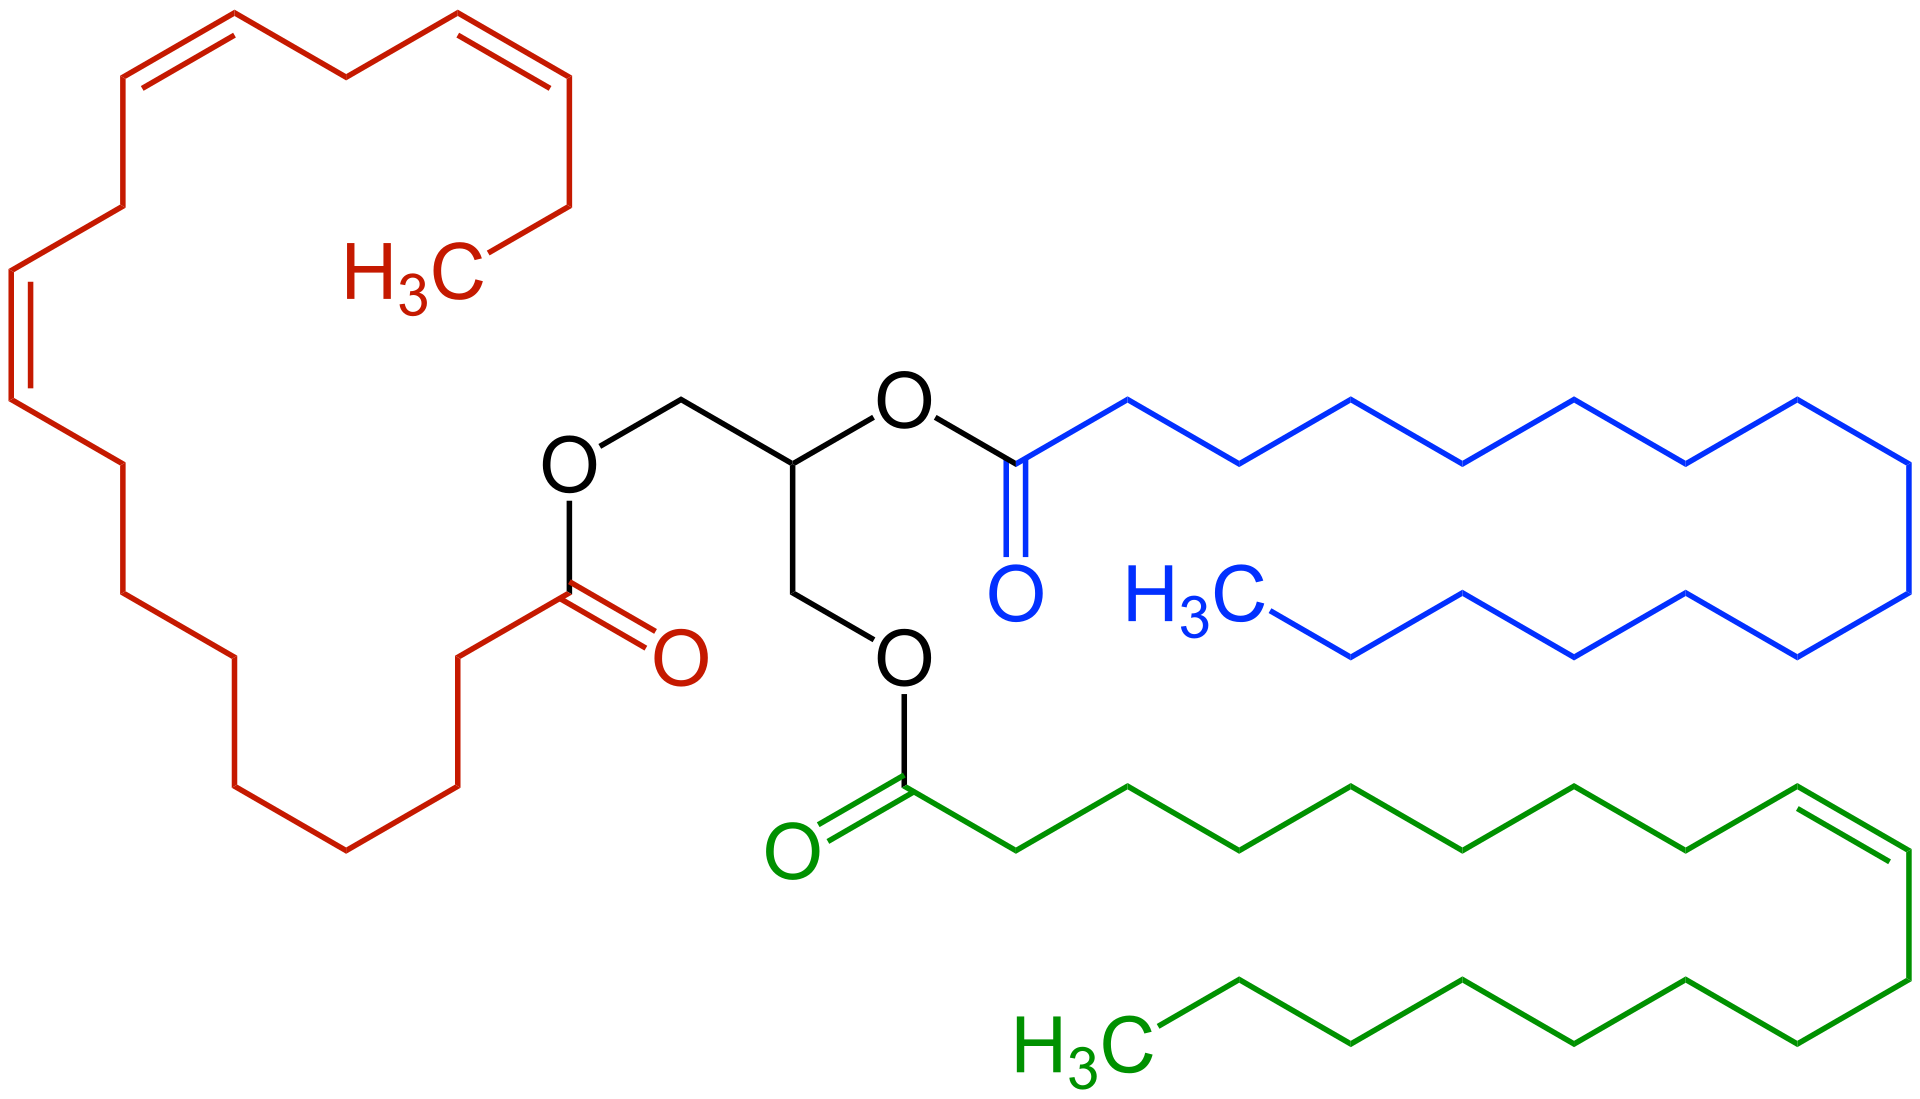
\includegraphics[width=10cm]{../images/Triglyzerid.png}
            \caption{Triglyzerid (blau: gesättigt, grün: einfach ungesättigt, rot: mehrfach ungesättigt)}
        \end{figure}

        \framebreak

        \begin{block}{Fakten}
            \begin{itemize}
                \setlength\itemsep{1em}
                \item Fett macht nicht fett
                \begin{itemize}
                    \setlength\itemsep{1em}
                    \item Nahrungsfett $\neq$ Körperfett
                    \item Hormonstörungen und Entzündungen machen dick und krank
                \end{itemize}
                \item Dosis und Qualität von Fettsäuren ist wichtig
                \begin{itemize}
                    \setlength\itemsep{1em}
                    \item "`Vorsichtige"' Herstellung
                    \item BIO-Siegel
                    \item Kaltpressung
                    \item Ausschluss von Licht, Hitze und Sauerstoff (Oxidation)
                \end{itemize}
                \item Fett macht schlau, schlank und gesund
            \end{itemize}
        \end{block}
    \end{frame}

    \subsection{Qualitätsmerkmale}
    \begin{frame}
        \frametitle{Qualitäten von Fett}
        \begin{block}{Die richtige Dosis und Qualität von Fetten führt zu\ldots}
            \begin{itemize}
                \setlength\itemsep{1em}
                \item exzelenter Energieversorgung
                \item vielfältigen Geschmäckern (Geschmacksträger)
                \item guter Vitaminversorgung
                \item langem, erfüllendem Sättigungsgefühl
            \end{itemize}
        \end{block}
    \end{frame}

    \subsection{Nahrungsfette}
    \begin{frame}[allowframebreaks]
        \frametitle{Nahrungsfette - Mindmap}
        \begin{figure}{}
            \centering
            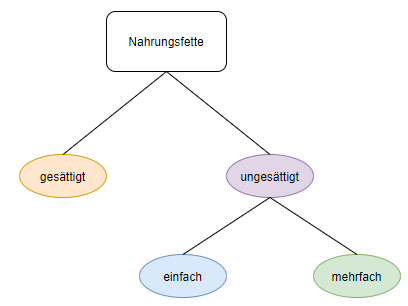
\includegraphics[width=5cm]{../images/Fette_Kategorisierung.png}
            \caption{Kategorisierung von Fettsäuren}
        \end{figure}

        \framebreak

        \begin{figure}
            \centering
            \includegraphics[width=8cm]{../images/Fette_Kategorisierung_gesättigt.png}
            \caption{Gesättigte Fettsäuren}
        \end{figure}

        \framebreak

        \begin{figure}
            \centering
            \includegraphics[width=8cm]{../images/Fette_Kategorisierung_ungesättigt.png}
            \caption{Ungesättigte Fettsäuren}
        \end{figure}

        \framebreak

        \begin{figure}
            \centering
            \includegraphics[width=8cm]{../images/Fette_Kategorisierung_ungesättigt_einfach_mehrfach.png}
            \caption{Einfach und mehrfach ungesättigte Fettsäuren}
        \end{figure}
    \end{frame}

    \subsection{Fettsäureprofile}
    \begin{frame}
        \frametitle{Fettsäureprofile}

        \begin{figure}
            \centering
            \includegraphics[width=10cm]{../images/Fettsäurenprofil_2.png}
            \caption{Fettsäureprofil einiger Fette}
        \end{figure}
    \end{frame}

    \subsection{N-kettige Fettsäuren}
    \begin{frame}[allowframebreaks]
        \frametitle{N-kettige Fettsäuren}

        \begin{block}{Kurzkettige Fettsäuren (SCFA = Short Chain Fatty Acids)\ldots}
            \begin{itemize}
                \setlength\itemsep{1em}
                \item werden von Bakterien im Darm gebildet unter Zufuhr von Ballaststoffen
                \begin{itemize}
                    \item Obst, Gemüse, Hülsenfrüchte, Kartoffeln, etc.
                \end{itemize}
                \item regulieren das Körpergewicht
                \item vermindern das Darmkrebsrisiko
                \item erhöhen Insulinempfindlichkeit
                \item sind entzündungshemmend
            \end{itemize}
        \end{block}

        \framebreak

        \begin{block}{Mittelkettige Fettsäuren (MCFA = Middle Chain Fatty Acids)\ldots}
            \begin{itemize}
                \setlength\itemsep{1em}
                \item sind gesättigt
                \begin{itemize}
                    \item Butter, Kokosfett, Palmfett, etc.
                \end{itemize}
                \item sind die "`Streber"' unter den Fettsäuren
                \item werden bei Darmerkrankungen genutzt
                \item sind pure Energie und werden in Mitochondrien zu Ketonen umgewandelt
                \item werden nicht gespeichert
                \item 8,3 kcal/g anstatt 9 ckal/g
            \end{itemize}
        \end{block}

        \framebreak

        \begin{block}{Langkettige Fettsäuren (LCFA = Long Chain Fatty Acids)\ldots}
            \begin{itemize}
                \setlength\itemsep{1em}
                \item sind z.B. einige Omega-3- und Omega-6-Fette
                \begin{itemize}
                    \item Ölsäure, Olivenöl, EPA, DHA
                \end{itemize}
            \end{itemize}
        \end{block}

    \end{frame}

    \subsection{Omega-Quotient}
    \begin{frame}[allowframebreaks]
        \frametitle{Omega-Quotient}

        \begin{figure}
            \centering
            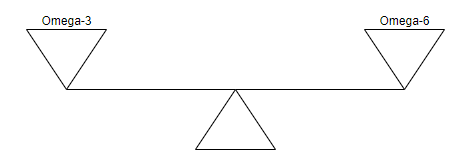
\includegraphics[width=4cm]{../images/omega-waage.png}
            \caption{Verhältnis von Omega-3- zu Omega-6-Fettsäuren}
        \end{figure}

        \framebreak

        \begin{block}{Ein gestörter Omega-Quotient führt langfristig zu\ldots}
            \begin{itemize}
                \setlength\itemsep{1em}
                \item Diabetes
                \item Krebs
                \item Herzinfakt
                \item Schlaganfall
                \item Demenz
                \item vorzeitiges Altern
                \item phsychischen Erkrankungen
            \end{itemize}
        \end{block}
    \end{frame}

    \subsection{Killerfette}
    \begin{frame}[allowframebreaks]
        \frametitle{Killerfette: Die Transfette (TFA = Trans Fatty Acids)}

        \begin{itemize}
            \setlength\itemsep{1em}
            \item Kommen nicht in der Natur vor
            \item Industriell gefertigt, erfunden im ersten Weltkrieg, Raffination
            \item Negativ-Rekorde für Transfett in
            \begin{itemize}
                \setlength\itemsep{1em}
                \item Backwaren, Kekse, Cracker, Chips, Pommes und Magerine
            \end{itemize}
            \item Transfette erkennen
            \begin{itemize}
                \setlength\itemsep{1em}
                \item "`gehärtet"', "`teilgehärtet"', "`raffiniert"'
            \end{itemize}
        \end{itemize}

        \framebreak

        \begin{block}{Diverse Studienergebnisse}
            \begin{itemize}
                \setlength\itemsep{1em}
                \item Transfette bei Affen führen zu Zellen, die Entzündungshormone produzieren
                \item Forschung warnt schon seit 1981 vor Transfetten und deren Auswikungen auf das Herz-Kreislauf-System
                \item Transfette führen zu Leaky Gut Syndrom, Darm- und Brustkrebs
            \end{itemize}
        \end{block}
    \end{frame}

    \section{Praxis}
    {
        \setbeamercolor{normal text}{fg=hBlue}\usebeamercolor*{normal text}
        \begin{frame}
            \begin{center}
                \Huge Praxis
            \end{center}
        \end{frame}
    }

    \subsection{Test}
    \begin{frame}
        \frametitle{Test}

        \begin{itemize}
            \setlength\itemsep{1em}
            \item Weniger industriell-verarbeitete Produkte
            \item Mehr Fett! (Kein Transfett)
            \item Kokosöl als Hand- und Gesichtscreme
            \item Ölziehen bei Zahn- und Zahnfleischproblemen
            \item Jeden Schritt der Verdauung mitnehmen!
        \end{itemize}
    \end{frame}

    \section{Fragerunde}
    {
        \setbeamercolor{normal text}{fg=hBlue}\usebeamercolor*{normal text}
        \begin{frame}
            \begin{center}
                \Huge Fragerunde
            \end{center}
        \end{frame}
    }

\end{document}